% !TEX TS-program = pdflatex
% !TEX encoding = UTF-8 Unicode

% This is a simple template for a LaTeX document using the "article" class.
% See "book", "report", "letter" for other types of document.

\documentclass[11pt]{article} % use larger type; default would be 10pt.
\setcounter{secnumdepth}{2}

\usepackage{paralist} % very flexible & customisable lists (eg. enumerate/itemize, etc.)

\usepackage{hyperref}

\usepackage[utf8]{inputenc} % set input encoding (not needed with XeLaTeX)
\usepackage{float} % to place float images correctly
\usepackage{color} % to color text
\usepackage{enumitem} % for lists
\usepackage{subfigure} % for mockups
\usepackage[font={it}]{caption} % for captions


%%% Examples of Article customizations
% These packages are optional, depending whether you want the features they provide.
% See the LaTeX Companion or other references for full information.

%%% PAGE DIMENSIONS
\usepackage{geometry} % to change the page dimensions
\geometry{a4paper} % or letterpaper (US) or a5paper or....
% \geometry{margin=2in} % for example, change the margins to 2 inches all round
% \geometry{landscape} % set up the page for landscape
%   read geometry.pdf for detailed page layout information

\usepackage{graphicx} % support the \includegraphics command and options

% \usepackage[parfill]{parskip} % Activate to begin paragraphs with an empty line rather than an indent

\usepackage{listings}
\usepackage{color}
 
\definecolor{codegreen}{rgb}{0,0.4,0}
\definecolor{codegray}{rgb}{0.5,0.5,0.5}
\definecolor{codepurple}{rgb}{0.58,0,0.82}
 
\lstdefinestyle{mystyle}{ 
    commentstyle=\color{magenta},
    keywordstyle=\color{blue}\bfseries,
    numberstyle=\tiny\color{codegray},
    stringstyle=\color{codepurple},
    basicstyle=\footnotesize,
    breakatwhitespace=false,         
    breaklines=true,                 
    captionpos=b,                    
    keepspaces=true,                 
    numbers=left,                    
    numbersep=5pt,                  
    showspaces=false,                
    showstringspaces=false,
    showtabs=false,                  
    tabsize=2,
   emph={self}, 
   emphstyle=\color{blue}, 
   emph={[2] BookingManager, FineManager}, 
   emphstyle=[2]\color{codegreen}\bfseries, 
   emph={[3]__init__, newBook, removeReservation, getReservation, manageExpired, min_heap, pop, now, timedelta, expireReservation}, 
   emphstyle=[3]\color{codegreen}, 
}
 
\lstset{style=mystyle}





%%% PACKAGES
\usepackage{booktabs} % for much better looking tables
\usepackage{array} % for better arrays (eg matrices) in maths
%\usepackage{paralist} % very flexible & customisable lists (eg. enumerate/itemize, etc.)
\usepackage{verbatim} % adds environment for commenting out blocks of text & for better verbatim
%\usepackage{subfig} % make it possible to include more than one captioned figure/table in a single float
% These packages are all incorporated in the memoir class to one degree or another...

%%% HEADERS & FOOTERS
\usepackage{fancyhdr} % This should be set AFTER setting up the page geometry
\pagestyle{fancy} % options: empty , plain , fancy
\renewcommand{\headrulewidth}{0pt} % customise the layout...
\lhead{}\chead{}\rhead{}
\lfoot{}\cfoot{\thepage}\rfoot{}

%%% SECTION TITLE APPEARANCE
\usepackage{sectsty}
\allsectionsfont{\sffamily\mdseries\upshape} % (See the fntguide.pdf for font help)
% (This matches ConTeXt defaults)

%%% ToC (table of contents) APPEARANCE
\usepackage[nottoc,notlof,notlot]{tocbibind} % Put the bibliography in the ToC
\usepackage[titles,subfigure]{tocloft} % Alter the style of the Table of Contents
\renewcommand{\cftsecfont}{\rmfamily\mdseries\upshape}
\renewcommand{\cftsecpagefont}{\rmfamily\mdseries\upshape} % No bold!

\newcommand{\pe}{PowerEnJoy }
\newcommand{\pecomma}{PowerEnJoy, }
\newcommand{\bul}[1]{\indent$\bullet$ #1\\}

\usepackage{listings}
\usepackage{pxfonts}
\usepackage{enumitem}
\usepackage{tabularx}
\usepackage{pdfpages}


\newcommand{\extInput}[3]{ #1:  \textbf{#2} \\ #3  }

\newcommand{\risk}[2]{  \textbf{Risk: #1 \newline Selected strategy:}	#2 }




\usepackage{amsmath}
\usepackage{graphicx}
\usepackage[colorinlistoftodos]{todonotes}



%%% END Article customizations

%%% The "real" document content comes below...



\begin{document}


\begin{titlepage}

\newcommand{\HRule}{\rule{\linewidth}{0.5mm}} % Defines a new command for the horizontal lines, change thickness here
\center % Center everything on the page

%	LOGO SECTION

\includegraphics[width=10cm]{../DOC/polimiLogoNome.png}\\[0.5cm] % Include a department/university logo
 
%	HEADING SECTIONS
%\textsc{\Large Politecnico di Milano}\\[1cm] % Name of your university/college
%\textsc{\large Software Engineering II} \\
%\textsc{\large A. Y. 2016/2017}


%	TITLE SECTION
%\HRule \\[0.4cm]
\\[2cm]
{ \Huge \bfseries \pe} \\[0.5cm] % Title of your document
{ \LARGE \bfseries Project Plan Document} \\[0.5cm]
{\large Version 1.0}
\\[2cm] 
%\HRule \\[1.5cm]

%	AUTHOR SECTION
\Large \emph{Authors:}\\
{\Large \textsc{Mosciatti}} Simone\\ % Your name
{\Large \textsc{Zanzottera}} Sara\\
\\[1cm]
\emph{Reference Professor:} \\
{\Large \textsc{Mottola}} Luca % Supervisor's Name

\vfill % Fill the rest of the page with whitespace

%	DATE SECTION
{\large January 22, 2017}

\end{titlepage}


\newpage
\tableofcontents
\newpage


\section{Introduction}

\subsection{Purpose and Scope}

The main purpose of this Project Plan Document is to assess the expected complexity of \pecomma, evaluate the risks related to the project, estimate costs and effort we expect will be required in order to develop our software successfully.

This document is also meant to provide some guidelines for the project manager to allocate budget and resources to the project, and to help defining a schedule for the development team.

We are using Function Points and COCOMO II analysis to estimate the size of the project, in terms of lines of code and costs and effort required to get the final product in time. 

Then we provide a tentative schedule and a Gantt covering all the activities required to complete the project, from the very first operation to the actual deployement, that should help the managers defining a schedule. We also describe the expected load allocation for the team members.

Finally we provide a risk analysis for the most probable setbacks the project may face, and provide some preventive measures that should be performed in order to prevent a later, not recoverable failure in providing a software matching the expectations, in terms of feature, quality of code, costs and timing.


\subsection{Definitions, Acronyms, Abbreviations}
 \begin{description}
	\item[RASD] Requirements and Specification Document.
	\item[DD] Design Document.
	\item[User] A customer of \pe using the service.
	\item[Staff Operator (Operator)] An employee of \pe which takes care of the cars.
	\item[Ride] The action of getting onboard of a \pe car, start its engine, drive to destination and park.
	\item[Issue] Any problem a car may incur in, or a user may face while using the service.
	\item[Nearby Cars] Available cars located within a maximum distance to a specific position.
	\item[Available Cars] Cars whose Availability Status is set to ``Available``.
	]\item[Booking (Reservation)] The act to reserve a car for a limited amount of time for future use by a user.
	\item[Driver] Whoever is driving a regularly booked \pe car.
	\item[Driving License] The state's issued driving license of the user.
	\item[Fine] A fine issued by the local law enforcing officers to a user while driving a \pe car. 
	\item[Safe Area] An parking area, predefined by the company, where is possible to safely park the cars of the \pe fleet.
	\item[Car's Onboard System] The controll system of the car that is able to exchange data with the central system and to relevate operation parameters.
	\item[Customer's App] An implementation of the system frontend tailored to the need of the customers.
	\item[Staff's App] An implementation of the system frontend tailored to the need of the staff.
	\item[Central System (Main Server)] The central system for \pe. All the command and all the data are streamed, analyzed and used here.
	\item[GPS]: Global Positioning System is a global navigation satellite system (GNSS) that provides location and time information in all weather conditions, anywhere on or near the Earth where there is an unobstructed line of sight to four or more GPS satellites.
	\item[Location] Pair of integer values as provided by GPS sensors.
	\item[Payment Method] Set of data relative to a credit card.
	\item[Identity ID] Personal code provided by local authorities to uniquely identify citizens.
	\item[Driving License ID] The unique code reported on every legal driving license.
	\item[Scanned License] An high quality image of the driving license acquired by the car's onboard system.
	\item[FP] Function Points.
	\item[ILF] Internal logic file
	\item[ELF] External logic file.
	\item[DBMS] Database Management System.
	\item[API] Application Programming Interface.
	\item[UI] User Interface.
	\item[UX] User Experience.
	\item[MVP] Minimum Viable Product.
	\item[M2M Communication] Machine to machine communication.
	\item[SLOC] Single Line of Code.
  \end{description}

\subsection{Reference Documents}
\begin{itemize}
	\item \textit{Assignments AA 2016-2017.pdf} (Assignments document given by the teacher)
	\item \textit{Reqiurements And Specification Document} (referring to this project)
	\item \textit{Design Document} (referring to this project)
	\item	Reference for Functional Point \url{https://web.archive.org/web/20160516160212/http://www.softwaremetrics.com/fpafund.htm}
  \end{itemize}




\newpage
\section{Project size, cost and effort}

\subsection{Size estimation}

Here we use the Function Point Approach to determine the size of the project.

Since we already have well defined components and the interaction of those components between external and internal actors, it seems natural to use the complexity of their interactions to determinate the Function Points for each component.

Provided that all the components have an intrisic, similar complexity, it is reasonable to assume that components that interact with few other components are quicker and simpler to develop. In our opinion the real complexity lies in the connection of components, not in the components themselves.

The complexity weights we use from now on are the following:
\begin{table}[h]
\centering
\bgroup
\def\arraystretch{1.5}%  1 is the default, change whatever you need
	\begin{tabular}{| c | c | c | c |}
	\hline
	Function Type & LOW & AVERAGE & HIGH \\
	\hline
	Internal Logical Files & 7 & 10 & 15 \\
	External Interface Files & 5 & 7 & 10 \\
	External Input & 3 & 4 & 6 \\
	External Inquiry & 3 & 4 & 6 \\
	External Output & 4 & 5 & 7 \\
	\hline
	\end{tabular}
\egroup
\caption{Function Point's complexity weights}
\end{table}


\subsection{Internal Logical Files}

All the internal files are stored in a database.

The model for our database was discussed in the Design Document, but we report again the diagram to simplify the discussion.

\begin{figure}[H]
	\centering
	\includegraphics[width=1\textwidth]{../Architecture/UML/ModelZoomComponents.png}
	\caption{Class Diagram of the Model.}
\end{figure}	

We are considering all the components of LOW complexity except for:
\begin{itemize}[noitemsep]
	\item BOOKING entity: HIGH complexity. it is the central entity in the whole application, with a lot of relationships with other components and very high insert rates.
	\item CAR entity: AVERAGE complexity. It has a relationship with BOOKING, but has a lot of very volatile fields and its update rates are very high.
\end{itemize}

\subsubsection{Total for IFL}
Total = 8 * 7 + 10 + 15 =  81


\subsection{External Interface Files}

The project involves 3 external data sources.

\begin{description}
	\item[stripe] We consider this service of AVERAGE complexity. They provide a very extensive set of endpoints, but the documentation is extremelly well done. In addition, we need to use only a small subset of the available endpoints and they provide several facilities to test the integration seamlessly.
	\item[linfo.io] We consider this service of LOW complexity. Its only end point requires two inputs (center of the circle and radius) and return a set of objects inside that circle.
	\item[truelicense.com] We consider this service of LOW complexity. Its APIs consist of only one single endpoint where to send an image, providing in output the number of the license of the input image, if valid.
\end{description}

\subsubsection{Total for EIF}
Total = 7 + 5 + 5 = 17

\subsection{External Input}

Following the list of functionalities provided in the Design Document, we identified the following External Input sources and assessed their complexity.

\subsubsection{USER Component}


\begin{description}
	\item \extInput
		{USER/Register}
		{AVERAGE}
		{Some information need to be validated and it is necessary to be sure of the uniqueness of the users.}
	\item \extInput
		{USER/\{Login/Logout\}}
		{LOW}
		{Only few check are necessary to LOG a user, such a validate the credentials.}
	\item \extInput
		{USER/SetPaymentMethod}
		{AVERAGE}
		{It is necessary to coordinate the changes with the external system of paymet (stripe).}

\end{description}

\subsubsection{GEOLOCATION Component}

\begin{description}
	\item \extInput
		{GEOLOCATION/AvailableCar}
		{HIGH}
		{It handle geolocation queries. Its complexity should be AVERAGE, but we will put more effort in developing general routines in order to lower the complexity of all the other functionality that requires geolocation queries.}
	\item \extInput
		{GEOLOCATION/Areas}
		{LOW}
		{We can reuse many routines from GEOLOCATION/AvailableCar to build this function with a minimum effort. On top of that, most of this work is delegate to the external service linf.io}
	\item \extInput
		{GEOLOCATION/Issues}
		{LOW}
		{We can reuse many routines from GEOLOCATION/AvailableCar to build this function with a minimum effort.}
	\item \extInput
		{GEOLOCATION/IsSafeArea}
		{LOW}
		{We can reuse many routines from GEOLOCATION/AvailableCar to build this function with a minimum effort.}

\end{description}

\subsubsection{POSITION Component}

\begin{description}
	\item \extInput
		{POSITION/Car}
		{AVERAGE}
		{This function requires the use of the car's onboard system and the communication system.}
	\item \extInput
		{POSITION/User}
		{LOW}
		{This function uses the GPS inside the user device, however it is a pretty standard, well known function.}
	\item \extInput
		{POSITION/Areas}
		{LOW}
		{Little more than a simple lookup in the database}
\end{description}

\subsubsection{BOOKING Component}

\begin{description}
	\item \extInput
		{BOOKING/Book}
		{LOW}
		{A simple write operation in the database. Most of the consistency checks are handled by the DBMS itself.}
	\item \extInput
		{BOOKING/Unbook}
		{LOW}
		{A simple update in the database. Most of the consistency checks are handled by the DBMS itself.}
	\item \extInput
		{BOOKING/Expire}
		{AVERAGE}
		{Other than modifying the database, this functionality needs to interact with the external payment system.}
\end{description}

\subsubsection{CAR Component}

\begin{description}
	\item \extInput
		{CAR/Unlock}
		{LOW}
		{Provided a reliable channel of communication with the car and a working on board system (assumption that I will keep for the rest of the documet), this functionality is a simple request to the car on board main system.}
	\item \extInput
		{CAR/ValidateLicense}
		{LOW}
		{Most of the work is handled by the external component truelicense.com}
	\item \extInput
		{CAR/Lock}
		{AVERAGE}
		{It is a simple command send to the car on board system. However, it has to trigger correctly the payment procedure starts.}
	\item \extInput
		{CAR/TurnOff}
		{LOW}
		{It is a simple command send to the car on board system.}
	\item \extInput
		{CAR/Telemetry}
		{HIGH}
		{By itself this component should have a LOW complexity. However, assigning a HIGH complexity we are considering the complexity of setting up a reliable communication channel between the main server and the cars.}
	\item \extInput
		{CAR/SetStatus}
		{LOW}
		{It is a simple update in the database.}
	\item \extInput
		{CAR/GetDetails}
		{LOW}
		{It is a simple read in the database. If data is too old, it also involves some communication from the server to the car, an operation still considered of LOW complexity.}
\end{description}

\subsubsection{RIDE Component}

\begin{description}
	\item \extInput
		{RIDE/Start}
		{LOW}
		{It simply performs an update in the database.}
	\item \extInput
		{RIDE/End}
		{LOW}
		{It simply performs an update in the database.}
\end{description}

\subsubsection{ISSUE\_MANAGER Component}

\begin{description}
	\item \extInput
		{ISSUE/New}
		{LOW}
		{It simply performs an update in the database.}
	\item \extInput
		{ISSUE/TakeCharge}
		{LOW}
		{It simply performs an update in the database.}
	\item \extInput
		{ISSUE/Solve}
		{LOW}
		{It simply performs an update in the database.}
	\item \extInput
		{ISSUE/GiveUp}
		{LOW}
		{It simply performs an update in the database.}
\end{description}

\subsubs
ection{Total for External Input}
Total = 18 * 3 + 6 * 6 + 2 * 6 =  102

\subsection{External Inquiry}

\subsubsection{RIDE\_MANAGER Component}
\begin{description}
	\item \extInput
		{RIDE/FindRides}
		{LOW}
		{It is a simple lookup in the database.}
\end{description}

\subsubsection{Total for External Inquiry}
Total = 1 * 3 = 3

\subsection{External Output}

\subsubsection{BILLING\_MANAGER Component}
\begin{description}
	\item \extInput
		{BILL/CalculateRideFee}
		{AVERAGE}
		{It require to know the overall time of the ride and the bonus and malus applied.}
	\item \extInput
		{BILL/CalculateExpireBookFee}
		{LOW}
		{It returns a constant value.}
	\item \extInput
		{BILL/CalculateUnsafeParkingFine}
		{LOW}
		{It returns a constant value.}
\end{description}

\subsubsection{NOTIFIER}
\begin{description}
	\item \extInput
		{NOTIFY/Notify}
		{AVERAGE}
		{This functionality takes care of different types of notification. It is not ``a size fits all''.}
\end{description}

\subsubsection{Total for External Output}
Total = 2 * 4 + 2 * 5 = 18

\subsection{Overall count}

The overal total is: 81 + 17 + 102 + 3 + 18 = 221 \newline
Lower bound of: 221 * 46 = {\Large 10166} lines of code \newline
Upper bound of: 221 * 67 = {\Large 14807} lines of code.




\newpage
\section{Cost Estimation COCOMO II}

In this section we are exploring the scale and the cost drivers for the COCOMO II model in order to find a reasonable timing for the project.

\subsection{Scale Driver}

Given the table listed in section 1.3: References Documents, we attribute the following values to the Scale Driver.

\begin{description}
	\item[PREC] (Precedentedness):  {\large 2.48} 
\\ The team is Generally familiar with the problem space. It has never built the same product before, but it built several part of it a lot of times.
	\item[FLEX] (Development Flexibility): {\large 2.03} \\ All the documents are written assuming that during the development phase a lot of unforeseeable issues would arise. We are expecting general conformity of the finished product to the designed one.
	\item[RESL] (Architecture / Risk Resolution): {\large 2.83} \\ In the following part of the document we present a quite comprensive risk mitigation strategy. 
	\item[TEAM] (Team Cohesion): {\large 1.10} \\ The team is highly cooperative. 
	\item[PMAT] (Process Maturity): {\large 3.12} \\ The team already works in the industry, knows and applies best practise.
\end{description}

\subsection{Cost Driver}

\begin{description}
	\item[RELY] (Required Software Reliability): {\large 1.00} \\ In case of the interruption of the service, there won't be heavy financial losses but only easily recoverable ones.
	\item[DATA] (Data Base Size): {\large N/A} \\ Our most populated table will have less than 100k rows on the foreseeable future. Given the lower bound of roughly 10k SLOC, our D/P ratio is of less than 10.
	\item[CPLX] (Product Complexity): {\large 1.00} \\ Our code does not present any over complex structure, we will set to nominal the overall complexity.
	\item[RUSE] (Developed for Reusability): {\large 1.00} \\ We are going to develop some functions for reusability across the project.
	\item[DOCU] (Documentation Match to Life-Cycle Needs): {\large 1.00} \\ We are keeping the documentation in sync with our software's releases.
	\item [TIME] (Execution Time Constraint): {\large 1.00} \\  The software is not particulary CPU bounded. We are expecting a fairly low use of CPU.
	\item[STOR] (Main Storage Constraint): {\large N/A} \\  Storage is not an issue for our application.
	\item[PVOL] (Platform Volatility): {\large 1.00} \\  We are going to base all our development stack on proven and widely used open source frameworks and components. We are conservatively setting this value to its nominal value.
	\item[ACAP] (Analyst Capability): {\large 0.85} \\  We are confident that we conducted a fairly comprensive analysis of the overall project and so we set this value to a pretty high value.
	\item[PCAP] (Programmer Capability): {\large 0.88} \\  We both have real word experience working in complex projects and in contributing to the open source.
	\item[PCON] (Personnel Continuity): {\large 0.81} \\  There will be no turnover.
	\item[APEX] (Applications Experience): {\large 0.88} \\  We chose technologies that we know and that we have already used before.
	\item[PLEX] (Platform Experience): {\large 0.91} \\  We chose the platform basing on our previous experience.
	\item[LTEX] (Language and Tool Experience): {\large 0.91} \\  We both have worked before with all the tools that we will need in the project as well as for the programming languange we selected.
	\item[TOOL] (Use of Software Tools): {\large 0.90} \\  We are going to automate as much as possible the lifecycle of the product.
	\item[SITE] (Multisite Development): {\large 0.86} \\  The team members are located in the same city and use all the technologies to communicate as much as possible.
	\item[SCED] (Required Development Schedule): {\large 1.00} \\ We don't plan to inpose any schedule constraint on the project.
\end{description}

The overall result of the analysis of the cost driver is summed up in the following table.

\begin{table}[h]
\centering
\bgroup
\def\arraystretch{1.5}%  1 is the default, change whatever you need
	\begin{tabular}{| c | c | c | c |}
	\hline
	RELY & Precedentedness & Nominal & 1.00 \\ \hline
	DATA & Development Flexibility & Very Low & n/a \\ \hline
	CPLX & Product Complexity & Nominal & 1.00 \\ \hline
	RUSE & Developed for Reusability & Nominal & 1.00 \\ \hline
	DOCU & Documentation Match to Life-Cycle Needs & Nominal & 1.00 \\ \hline
	TIME & Execution Time Constraint & Nominal & 1.00 \\ \hline
	STOR & Main Storage Constraint & Low & n/a \\ \hline
	PVOL & Platform Volatility & Nominal & 1.00 \\ \hline
	ACAP & Analyst Capability & High & 0.85 \\ \hline
	PCAP & Programmer Capability & High & 0.88 \\ \hline
	PCON & Personnel Continuity & Extra High & n/a \\ \hline
	APEX & Applications Experience & High & 0.88 \\ \hline
	PLEX & Platform Experience & High & 0.91 \\ \hline
	LTEX & Language and Tool Experience & High & 0.91 \\ \hline
	TOOL & Use of Software Tools & High & 0.90 \\ \hline
	SITE & Multisite Development & Very High & 0.86 \\ \hline
	SCED & Required Development Schedule & Nominal & 1.00 \\ \hline \hline 
	\multicolumn{3}{| c |  }{Product} & 0,422 \\ \hline
	\end{tabular}
\egroup
\caption{Results of the analysis of cost drivers}
\end{table}




\clearpage
\section{Effort Estimation}

Given the above points, we can estimate the required effort in Person-Month (PM).

We use the following formula:

$$ \text{Effort} = A * EAF * KSLOC ^ E $$

Using the following substitutions:

$$ A = 2.94 $$
$$ EAF = 0.422 $$
$$ E = B + 0.01 * sum(scale driver) $$

we get E equals to: 

$$ E = 0.91 + 0.01 * 11.56 = 0.91 + 0.1156 = 1,0256 $$

that leads us to the evaluations listed in table 3.

Now we calculate F as:

$$ F = 0.28 + 0.2 * (E - B) = 0.28 + 0.2 * (1.0256 - 0.91) = 0.303 $$

allowing us to determine also the duration's upper and lower bounds, also listed in Table 3.

\begin{table}[h]
\centering
\bgroup
\def\arraystretch{1.5}
	\begin{tabular}{| c | c | c |}
	\hline
	Lower Bound & 2.94 * 0.422 * 10.166 ** 1.0256 & 13.38 \\ \hline
	Upper Bound & 2.94 * 0.422 * 14.807 ** 1.0256 & 19.68 \\ \hline \hline
	Duration & 3.67 * Effort ** F & ? \\ \hline \hline
	Duration Lower Bound & 3.67 * 13.38 ** 0.303 & 8.05 \\ \hline
	Duration Upper Bound & 3.67 * 19.68 ** 0.303 & 9.05 \\ \hline
	\end{tabular}
\egroup
\caption{Effort Estimates}
\end{table}




\newpage
\section{Schedule}

Given that most of the analysis is already done, we are going to focus on the development schedule and the deployement of the software.

\subsection{Timespan of the project development}
Our risk mitigation strategy requires us to validate the product as early as possible. This request dictates slower development cycles, but ensures the quality of the final result we are getting, which is very relevant also from a business perspective. 

We can accept a slower development schedule, since our time estimation are quite short. Nevertheless we account for an additional month of time, bringing the total time of development to roughly 10 person months.

We believe this is a reasonable tradeoff between the use of time and the risk management.

\subsection{Deployement stages}
The very first step consists in developing a very simple MVP that selected alpha users can use to rent cars once or twice a day for a small nominal fee. 

A careful selection of the alpha testers should prevent the cars from being damaged, and prevent abuses on the alpha version of the system. At the same time, this process provides us extremelly valuable feedback on the system we are building and the interaction with the users.

During the MVP phase, techinical staff should be always present in order to manually fix any kind of problem that may arise.

After this phase, if the stackholders of the project agree, we proceed with the creation of the real platform and we decide what components of the MVP to keep (if any). The experience gained building the MVP will be extremelly valuable also after this phase, because will let us moving very fast and with confidence. During this phase we develop also the unit and the integration tests.

We aim to keep a clean building/deploy pipeline. In this way we can always deploy our platform. Keeping such pipeline is expensive and time consuming, but it provides a lot of benefits. With a clean pipeline we can:

\begin{enumerate}[noitemsep]
	\item Mirror the alpha traffic to the new service.
	\item Move alpha users to the new service and effectively make them beta users.
	\item Add more beta user to the service.
\end{enumerate}

Using this approach the developing time will be a little longer, but we are keeping the risk as low as possible. We can afford this since our design is extremely decoupled and simple to build, so our developing time is short.

\subsection{Detailed Schedule}
\begin{figure}[H]
	\centering
	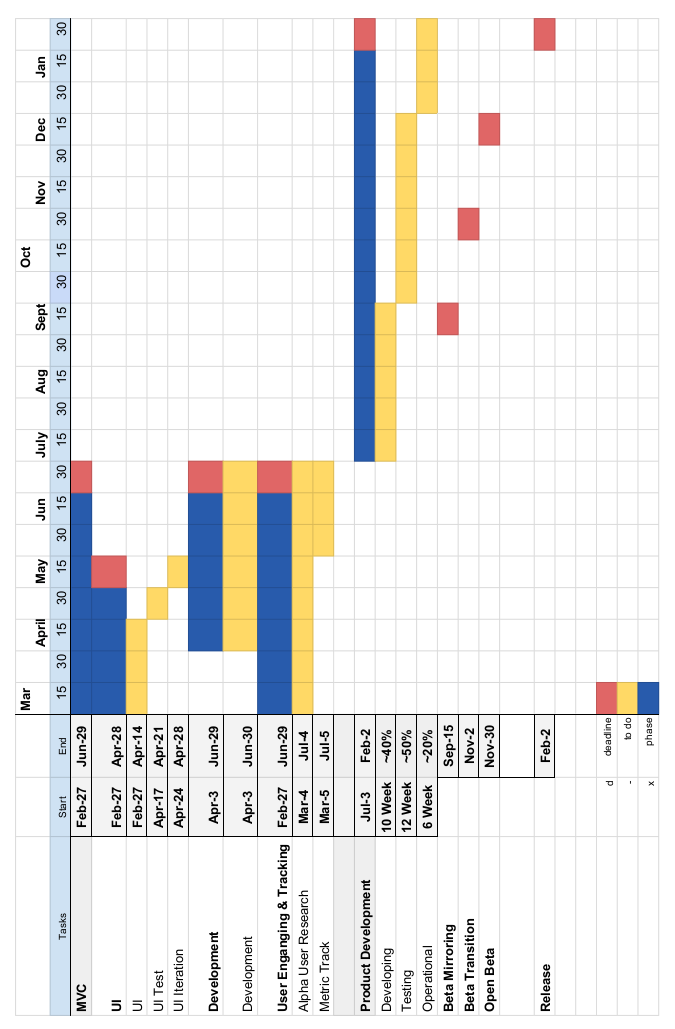
\includegraphics[width=0.8\textwidth]{GANTT/GANTT.png}
	\caption{Gantt Chart for \pe}
\end{figure}	

In the above Gantt chart we did not actually specified what time slot is associated with which activity. We simply gave an estimate of the time percentage each activity should take on the whole time period.

This approach is required since all the activities on each module should procede in parallel with code and tests development, while the setting of the operational activity is set to start shortly thereafter.

These methodologies help us incorporating the feedback from both the user and the test environment as soon as possible during the development cycle. 

For example, we may discover that the user is eager to pay something to keep the car booked for more time than a single hour: using this method we will be able to incorporate such feedback immediately in the system.
Moreover, if we discover that some of our modules are not able to keep up with the expected load, we could immediately allocate more resources and time to fix that side of the project.


\newpage
\section{Resource Allocation}

Our small team's members have different and complementary skill.

Sara is more experienced in UI / UX and in clearly communicating with the stackholders; Simone is more experience in backend developing and M2M communication.

Both of us have a fairly good generic programming experience.

Since the components are already defined, as well as their interface, only a single developer will be responsible for every single component.

In order to fairly allocate the several components to each developer, we use the complexity factor calculated above.

Given the different skills and experience of the developing team members, the two developer are allocated to the different modules in the following way:

\begin{description}
	\item[Simone] \hfill
		\begin{enumerate}
			\item GEOLOCATION
			\item POSITION
			\item CAR
			\item RIDE
		\end{enumerate}
	\item[Sara] \hfill
		\begin{enumerate}
			\item USER
			\item BOOKING
			\item ISSUE
			\item BILL
			\item NOTIFY
			\item User Interface
		\end{enumerate}
\end{description}

In this way both developers will handle closely related modules while working in the field they know best.

\begin{comment}
L = 3
A = 4
H = 6

USER -> 11
GEOLOCATION -> 15
POSITION ->10
BOOKING -> 10
CAR -> 25
RIDE -> 6 + 3
ISSUE -> 13
BILL -> 13
NOTIFY -> 5

SIMO -> GEOLOCATION + POSITION + CAR + RIDE = 15 + 10 + 25 + 9 = 59
SARA -> USER + BOOKING + ISSUE + BILL + NOTIFY = 11 + 10 + 13 + 13 + 5 = 52
\end{comment}





\newpage
\section{Risk Management}

In the following section we list the possible risks that can determine the failure of our project, and we set a strategy to prevent each of them.

\subsection{Risks and Selected Stretegies}

\begin{enumerate}
	\item  \risk{ Users don't understand the User Interface}
			{\begin{itemize}[noitemsep, nolistsep]
				\item Adopt standard symbols and icon
				\item Test first mock up of the UI with target demography
			\end{itemize} }
	\item  \risk{ Software more complex than our estimation}
			{\begin{itemize}[noitemsep, nolistsep]
				\item Set several milestones along the development process, so to catch as early as possible if the project is going to run late. 
			\end{itemize} }
	\item  \risk{ Users don't like the product}
			{\begin{itemize}[noitemsep, nolistsep]	
				\item Provide a MVP.
				\item Get feedback from the market as soon as possible. \newline( It is fine to loose money during this phase).
			\end{itemize} }
	\item  \risk{ Low Quality software}
			{\begin{itemize}[noitemsep, nolistsep]
				\item Automatic test regarding both performance and corecteness.
			\end{itemize} }
\end{enumerate}





\newpage
\section{Conclusions}

\subsection{Tools used}
During the development of this document we used the following tools:
\begin{itemize}
	\item \textbf{Github} to version control the project
	\item \textbf{\LaTeX} on TeXworks to redact this document
	\item \textbf{GoogleDocs} to redact the Gantt diagram
\end{itemize}

\subsection{Hours of work}
\begin{itemize}
	\item SM: 5h on 16/01
	\item SZ: 5h on 16/01
	\item SM: 7h on 17/01
	\item SZ: 2h on 17/01
	\item SM: 3h on 18/01
	\item SZ: 2h on 18/01
	\item SZ: 1h on 22/01
\end{itemize}





\end{document}